\chapter{Cylindrical Simulations to Study the Effect of Beam Radius in Direct-Drive}

This chapter describes a cylindrical, direct-drive implosion simulation platform and corresponding ensemble of simulations that was developed to study the effect of the beam radius initial condition on \textsc{Omega} laser facility experiments.
Although results from the cylindrical simulations do not have the same convergence properties of spherical implosions, much of the essential physics which is important to studying the effect of beam radius is preserved.
The main benefit of the geometry is that a 2-D ray-trace can be used to model the lasers which yields several orders of magnitude speed up, compared to spherical 3-D implosions.
The reduction in computational expense allows ensembles of \ac{CBET} simulations to be performed, which would be exceedingly expensive for 3-D spherical calculations.
Beam radius strongly effects \ac{CBET} and therefore including a model for the interaction in computational studies is crucial.

The chapter begins with a review of the work which has been done to study the beam radius initial condition for direct-drive implosions, with an emphasis on the use of this parameter in statistical modelling of \textsc{Omega} campaigns.
A description of the cylindrical platform is then provided, which includes a discussion of its advantages, weaknesses and applicability to current \textsc{Omega} experiments.
The tuning procedure which was followed to obtain hydrodynamically similar implosions at different beam radii is then described.
The main results of the chapter are then presented, which include calculations of the power deposition asymmetry both with and without \ac{CBET} and an explanation of why \ac{CBET} typically amplifies the asymmetry.
\ac{CBET} is also shown to introduce \textit{modal flips} of the deposition in time.
Stagnation state asymmetries of the hydrodynamic profiles are then studied for all implosions and these demonstrate that while increasing beam radius in the absence of \ac{CBET} reduces beam mode asymmetries, the opposite behaviour is observed in the presence of \ac{CBET}, although the exact relationship proves is complex.
The chapter concludes with a summary of the work and suggestions of further work that could be undertaken using the same cylindrical platform.

\newpage

%###############################################################################################################################
%###############################################################################################################################
%###############################################################################################################################
\section{Introduction to Beam Radius in Direct-Drive Inertial Confinement Fusion}%
\label{sec:Res1_Beamrad_intro}

\begin{figure}[t!]
    \includegraphics[width=\linewidth]{Results1/Images/RbRt_beam_overlap_alt.png}
    \centering
    \caption{The trajectory of rays from two beams with Beam radii.
    The density profile for both simulations is $n_e=n_{\text{cr}}\exp{[ -(r_{\mu\text{m}}-20)/100 ]}$.
    Panels a) and b) plot rays from beams with widths $\sigma=10$ and $18\ \mu\text{m}$ respectively.
    Ray trajectories are separated for each beam by colour depending on their sheet.
    Red and dark blue rays are from the incident sheet (before the ray caustic) and magenta and light blue rays are from the reflected sheet (after the ray caustic).}%
    \label{fig:Res1_RbRt_beam_overlap}
\end{figure}

An idealised direct drive implosion, (neglecting the effect of random or otherwise, shot-to-shot variations) has a limited number of initial conditions which define the implosion.
The target can be described by a set of materials and their thicknesses.
Initial target parameters are intimately coupled to the physics of the implosion and, in part, dictate the propagation time of shocks through the target, hydrodynamic stability and absorption of the laser energy.
The pulse shape describes the laser power which is incident of the target as a function of time.
This can be designed to, for example, drive shocks by introducing sharp rises in the incident power with time, which leads to sharp gradients in ablation pressure~\cite{scott_shock-augmented_2022}.
A given facility also has a number of beam ports each of which has a specific origin and pointing location, which influence the magnitude of the \textit{beam mode} asymmetry, which arises from the uniformity of laser absorption.
The intensity profile of each laser and specifically the beam radius is an additional parameter which can be varied and plays an important role in defining both the power which can be coupled to the target and the magnitude of beam mode asymmetry.

As shall be explored in this chapter, increasing the beam radius alters the magnitude of energy lost via \ac{CBET} leading to a reduction in the maximum target mass that can be imploded at a given speed
The beam radius relative to the target is therefore often effectively varied from shot to shot by changing the outer radius (and therefore mass) of the target.
This defines a dimensional variable, which is the radius of the beam divided by the target radius, $R_b/R_t$.
Typically, at the \textsc{Omega} laser facility, this is explicitly defined as the radius of the beam which contains 95 \% of the incident power divided by the initial outer target radius~\cite{froula_increasing_2012,colaitis_exploration_2023,anderson_enhanced_2024},
\begin{equation}
    R_b/R_t = \frac{r_{95}}{R_t},
\end{equation}
where $r_{95}$ is defined by the integral,
\begin{equation}
    \int_0^{r_{95}}e^{- \left| \frac{r}{\sigma} \right| ^{n_s}}\text{d}r = 0.95,
\end{equation}
and the definition of a circular, super-Gaussian beam profile from Eq.~\ref{eq:supgaus} has been used.
In the absence of \ac{CBET} it can intuitively be understood that increasing this parameter should improve the uniformity of the laser illumination, because beam spots overlap each other more on the target, and therefore reduce the beam mode~\cite{lees_understanding_2023}.
Larger $R_b/R_t$ also lead to slightly less absorption in the absence of \ac{CBET}, because a larger fraction of the incident light (especially at late time as the target converges) would reach lower density plasma and therefore not be absorbed.
\ac{CBET} significantly complicates this interpretation, however.

Fig.~\ref{fig:Res1_RbRt_beam_overlap}.a and Fig.~\ref{fig:Res1_RbRt_beam_overlap}.b plot results of a ray tracing calculation with a direct-drive relevant, exponentially decaying plasma density with a smaller and larger beam respectively.
In direct-drive, backscatter \ac{CBET} is the dominant mechanism which depletes absorption, which is where outbound light gains energy from inbound light\footnote{Note here that outbound here means light travelling quasi-parallel to the approximately radially outward fluid velocity and inbound means quasi-anti-parallel.}.
The outward rays from the small beam radius simulation in Fig.~\ref{fig:Res1_RbRt_beam_overlap}.a do not overlap the incident light from the other beam and therefore limited \ac{CBET} between these beams will occur.
The trajectories from the larger radius simulation in Fig.~\ref{fig:Res1_RbRt_beam_overlap}.b, however do cross the inbound rays from the other beam, which could lead to a resonant \ac{CBET} interaction, and significant reduction of the absorbed power.
As was shown in Fig.~\ref{fig:SOLAS_qpR_IFRIIT_test}, \ac{CBET} also substantially increases absorption asymmetry on the \textsc{Omega} laser facility.
This means that in the presence of \ac{CBET}, the effect of increasing $R_b/R_t$ on illumination asymmetry is not clear.
While in the absence of \ac{CBET}, it should lead to greater beam overlap, this increased overlap will result in more \ac{CBET} which could reduce uniformity of absorption.

Isolating the contribution of \ac{CBET} is of particular importance to allow extrapolation of experimental results to future facilities, because it is hoped that adding bandwidth to lasers will almost entirely eliminate \ac{CBET} scattering.
Studying which of these effects dominates is difficult to do experimentally, as significant backscatter \ac{CBET} occurs at all laser facilities which are capable of conducting compression experiments.
Therefore, computational studies are well suited to investigate how $R_b/R_t$ influences performance and the role of \ac{CBET} in this scaling.


%################################################################################
%################################################################################
\subsection{Previous Work Studying the Effect of $\mathbf{R_b/R_t}$ on \textsc{Omega}}%
\label{sec:Res1_OMEGA_stat_modelling_RbRt}

\begin{figure}[t!]
    \includegraphics[width=0.5\linewidth]{Results1/Images/RbRt_froula.png}
    \centering
    \caption{Soft x-rays emitted from the ablation surface of direct-drive implosions with various $R_b/R_t$ values, as measured by an x-ray framing camera.
    All images are taken at a constant capsule radius of $R=175\ \mu\text{m}$.
    The figure has been reproduced with permission from Ref.~\cite{froula_increasing_2012}.}%
    \label{fig:RbRt_froula}
\end{figure}

A great deal of experimental and computational work has been conducted to explore the effect that the beam radius has on direct-drive implosions.
Froula \text{et al.} conducted a series of implosions which systematically varied $R_b/R_t$ to explore the balance between increased \ac{CBET} at larger beam radii, which reduced the coupled energy and increased illumination non-uniformity at lower radii \cite{froula_increasing_2012}.
Soft x-ray emission data from a selection of implosions with different radii are plotted in Fig.~\ref{fig:RbRt_froula}, all of which are taken at the same convergence shell radius of the target as it implodes inwards.
These images show that at lower values of $R_b/R_t$, mid-mode perturbations\footnote{In direct-drive, \textit{mid-modes} are loosely defined as modes similar to $\ell=10$.} become increasingly significant.
The results of these experiments found that neutron yield was maximised at $R_b/R_t\sim 0.8$.
1-D modelling using the \ac{CBET} model in \textsc{Lilac} was in good agreement with the experimental results, verifying that \ac{CBET} was responsible for the decrease in coupled energy to the target~\cite{igumenshchev_crossed-beam_2012}.

%################################################################################
%################################################################################
\subsection{Statistical Modelling of \textsc{Omega} Direct-Drive Implosions}%
\label{sec:Res1_OMEGA_stat_modelling}

In recent years, a lot of work has been carried out to develop a statistical modelling capability for direct-drive implosions on the \textsc{Omega} laser facility.
This modelling serves several critical purposes including enhancing the predictive capability of simulations~\cite{lees_experimentally_2021}, guiding experimental design to achieve higher performance implosions~\cite{gopalaswamy_tripled_2019}, identifying important sources of degradation on current facilities~\cite{lees_understanding_2023,gopalaswamy_using_2021} and validating simulation codes to help ensure they produce physically relevant results~\cite{ejaz_deep_2024}.
The first generation statistical model, described by Lees \textit{et al.} in Ref.~\cite{lees_experimentally_2021}, created a mapping between experimental and 1-D simulation results in order to explain significant differences in their results.
1-D simulation results are fed into the model and degraded by a series of power law multiplications, which returns a more physically accurate experimental yield.
Each power law multiplication represents a physical process for yield degradation with respect to 1-D physics, not included in the simulation.
Each of these is termed a \textit{yield over clean} ($\text{YOC}_i$), where the $i$ refers to the different physical processes included in the model.
The neutron yield from the 1-D simulation ($\text{Y}^{\text{sim}}_{1\text{-D}}$) can thus be converted to a prediction of the experimental yield~\cite{lees_experimentally_2021},
\begin{equation}
    \text{Y}^{\text{exp}} = \left( \text{YOC}_h \text{YOC}_f \text{YOC}_{\ell=1} \text{YOC}_b \text{YOC}_{\text{res}} \right) \text{Y}^{\text{sim}}_{1\text{-D}},
\end{equation}
where $\text{YOC}_h$ is a degradation term from hydrodynamics and instability growth, $\text{YOC}_f$ is degradation due to radioactive decay of the Tritium fill, $\text{YOC}_{\ell=1}$ is degradation from $\ell=1$ modes, $\text{YOC}_b$ is degradation from finite number and radius of beams and $\text{YOC}_{\text{res}}$ is a residual size scaling which is required to reduce performance of hydrodynamically downscaled implosions~\cite{thomas_quantifying_2020}.
Each of these terms and their functional forms shall be discussed briefly, in order to provide context for the utility of the model and highlight that understanding the relevant physical processes which lead to degradation can improve its performance.

\paragraph*{Hydrodynamic Degradation}
1-D simulations do not capture short wavelength perturbations which grow via the \ac{RTI} and reduce the yield of experiments by puncturing and breaking up the shell as the capsule implodes inwards.
Instabilities may be seeded by laser imprint or small scale defects in the target materials.
Degradation can be reduced by altering implosion design to increase the shell adiabat which increases the ablative stabilisation of the \ac{RTI}, or by lowering the \ac{IFAR}, which increases the distance that the instability must grow through to puncture the shell.
Scaling with the target convergence ratio, $C_R\equiv R_0/R_{\text{stag}}$, is included along with the ratio of outer to inner shell radius, $\hat{D}\equiv R_{\text{out}}/R_{\text{in}}$, which is believed to compensate for inaccuracies in modelling the shock propagation speed through the target.
The hydrodynamic degradation term thus has the functional form,
\begin{equation}
    \text{YOC}_h = \left[ \frac{\left( \alpha/3 \right)^{1.1}}{\text{IFAR}/20} \right]^{\mu_1} C_R^{\mu_2} \hat{D}^{\mu_3},
\end{equation}
where the $\mu_i$ fitting parameters, which are obtained from nonlinear regression across many \textsc{Omega} shots.
The fitting procedure demonstrated that experimental yields are very significantly reduced by these hydrodynamic degradations, with the most unstable shots yielding values of $\text{YOC}_h\sim 0.1$ \cite{lees_understanding_2023}.

\paragraph*{Fill Age Degradation}
\textsc{Omega} cryogenic implosions contain a DT fuel gas fill with a surrounding ice layer.
The tritium in this fuel in unstable and undergoes radioactive decay to ${}^{3}\text{He}$ over the period of days to weeks which typically pass from initial gas filling to shot day~\cite{regan_national_2019}.
${}^{3}\text{He}$ has a lower freezing temperature than DT and thus sublimates, accumulating in the fill region.
The accumulation of Helium in the gas reduces the final yield both by increasing radiative losses due to its higher ionisation, and by increasing density of the vapour, reducing compressibility and thus decreasing stagnation pressure in the hot-spot.
Both of these effects can be captured by conducting 1-D simulations with a ${}^{3}\text{He}$ concentration (and corresponding reduction of tritium density) which is a function of fill age.
The yield over clean due to the fill age and radioactive decay can then be taken as the ratio of these 1-D simulation yields,
\begin{equation}
    \text{YOC}_h = \left( \frac{\text{Y}^{\text{sim}}_{1\text{-D,He}}}{\text{Y}^{\text{sim}}_{1\text{-D}}} \right)^{\mu_4},
\end{equation}
where $\text{Y}^{\text{sim}}_{1\text{-D,He}}$ is the yield from the 1-D simulation with accumulated ${}^{3}\text{He}$ and $\mu_4$ is a fitting parameter.
Good agreement is observed with a fitted parameter value of $\mu_4 = 1.3$.
The value is larger than 1 (and the 95 \% confidence interval does not include 1), which suggests stronger degradation than observed in 1-D calculations.
This could be due to radioactive decay damaging the shell and leading to hydrodynamic instability growth~\cite{lees_understanding_2023}.

\paragraph*{Mode 1 Degradation}
In direct-drive implosions on the \textsc{Omega} facility, $\ell=1$ modes can be introduced to an implosion by a global offset of the target from the target chamber centre, mispointing of the laser beams or a power imbalance.
These are random and uncontrollable and therefore the statistical models can only account for their effect after the shot has occurred, returning an estimated yield which could have been achieved if no $\ell=1$ were present, $\text{Y}^{\text{exp}}/\text{YOC}_{\ell=1}$.
Mode 1 asymmetries have a clear signature in the broadening of the neutron time-of-flight detector peaks, when observed from orthogonal lines of sight.
The width of the peaks from multiple lines of sight can be analysed to return an angularly resolved apparent ion temperature map~\cite{mannion_mitigation_2021}, the asymmetry of which is dominated by the lowest mode of the hot-spot~\cite{woo_inferring_2020}.
Thus, it is deduced that the ratio of the maximum to minimum apparent ion temperatures from the experimental neutron time-of-flight signal can be used as a proxy for the amplitude of the mode 1, $R_T = T_{\text{max}}/T_{\text{min}}$.
This leads to a yield over clean expression for the $\ell=1$ degradation source,
\begin{equation}
    \begin{gathered}
        \text{YOC}_{\ell=1} = \hat{R}_T^{\mu_5}, \\
        \hat{R}_t \equiv \max \left( \, \frac{R_T}{R_T^{\text{min}}} \right),
    \end{gathered}
\end{equation}
where $\mu_5$ is the fitting parameter and the minimum threshold value, $R_T^{\text{min}}$ is introduced due to imperfect reconstruction of the apparent ion temperature map and fitted separately.
Work has been conducted to minimise the effect of the $\ell=1$ on \textsc{Omega} by repositioning the target after several initial shots to minimise the asymmetry in the apparent ion temperature measurement and thus increase performance~\cite{mannion_mitigation_2021}.

\begin{figure}[t!]
    \includegraphics[width=0.7\linewidth]{Results1/Images/RbRt_degradation_Lees.jpeg}
    \centering
    \caption{Experimentally inferred fusion yield degradation due to the finite beam source on the \textsc{Omega} laser facility.
    The dotted orange curve is the fit obtained from just using the $\overline{R}_{b/t}$ relation, while the black dashed curve uses the full relation in Eq.~\ref{eq:Res1_RbRt_degradation}.
    The vertical dotted line indicates the critical threshold, $\hat{R}_{b/t}^{\text{crit}}=0.86$, after which the $\hat{R}_{b/t}$ also has an effect.
    The cross validation error from the $\overline{R}_{b/t}$ and full fit is $-1.0\ \%$ and $-0.5\ \%$ respectively.
    The figure has been reproduced with permission from Ref.~\cite{lees_understanding_2023}.}%
    \label{fig:RbRt_YOC_lees}
\end{figure}

\paragraph*{Finite Beam Degradation}
The \textsc{Omega} laser facility has 60 beams arranged around a sphere which gives generally good illumination uniformity on a hard sphere surface, less than the 1 \% deviation which is believed to be necessary to achieve ignition~\cite{craxton_direct-drive_2015,goncharov_national_2017}.
An $\ell=10$ remains in the deposition however, as is demonstrated in Fig.~\ref{fig:SOLAS_qpR_IFRIIT_test}, which is often referred to as the beam-mode.
In the absence of \ac{CBET}, increasing $R_b/R_t$ increases the hard-sphere illumination uniformity~\cite{gopalaswamy_using_2021}.
As already described however, increasing beam radius allows leads to more blowby light and therefore more \ac{CBET}.
This reduces the coupled energy and potentially introduces additional asymmetry to the implosion.
Additionally, increasing the overlap of beams on the target could reduce the amplitude of the imprint seed and therefore increase performance.
The uncertainty as to which physical mechanisms are important, is highlighted by the complexity of the degradation parameter,
\begin{equation}
    \label{eq:Res1_RbRt_degradation}
    \begin{gathered}
        \text{YOC}_{b} = \left( \overline{R}_{b/t} \right)^{\mu_6} \left( \hat{R}_{b/t} \right)^{\mu_7}, \\
        \overline{R}_{b/t} =
        \begin{cases}
            R_b/R_t & \text{if } R_b<R_t, \\
            1 &  \text{if } R_b\geq R_t,
        \end{cases} \\
        \hat{R}_{b/t} =
        \begin{cases}
            \frac{R_b}{R_t R_{b/t}^{\text{crit}}} & \text{if } R_b/R_t < R_{b/t}^{\text{crit}}, \\
            1 & \text{if } R_b/R_t \geq R_{b/t}^{\text{crit}},
        \end{cases} \\
    \end{gathered}
\end{equation}
where $\mu_6$ \& $\mu_7$ are fitting parameters, the threshold behaviour in $\overline{R}_{b/t}$ was chosen to fit a small number of shots ($<10$) at $R_b/R_t>1$ and the threshold behaviour at $R_{b/t}^{\text{crit}}$ was introduced to fit a physically unexplained transition between two regimes in the data.

The fitted curve from the model is shown in Fig.~\ref{fig:RbRt_YOC_lees}, as the black dashed curve alongside the inferred values from experimental data points.
Also plotted in orange is a fitted curve obtained from just using the simple $\overline{R}_{b/t}$ degradation.
Introducing the $R_{b/t}^{\text{crit}}$ threshold significantly reduces the cross validation error of the fir 
The switch between the two regimes is found from the fitting procedure to occur at $R_{b/t}^{\text{crit}}=0.86$.
This is close to value of minimum illumination asymmetry for beams incident on a hard hard-sphere ($R_b/R_t=0.82$), which suggests that the degradation at the lowest values of $R_b/R_t$ is dominated by beam-mode, however this has not been experimentally or computationally verified.
Experiments between $R_{b/t}^{\text{crit}} < R_b/R_t < 1$ could be influenced by changing behaviour due to \ac{CBET} or imprint, which is not properly captured by the 1-D \textsc{Lilac} simulations included in the model.

The hypothesis tested in this chapter is that the change in yield over clean at $R_b/R_t = R_{b/t}^{\text{crit}}$ is due to increasing \ac{CBET} as beam radius increases, which increases beam mode asymmetry and therefore suppresses the $\text{YOC}_{b}$ term.
Although \textsc{Lilac} does include a model for \ac{CBET}, it is a 1-D code and therefore the 3-D beam mode perturbations cannot be inferred from its results.
Qualitatively, this hypothesis can explain the observed behaviour in Fig.~\ref{fig:RbRt_YOC_lees}, which demonstrates that at $R_{b/t}^{\text{crit}}$, the gradient of $\text{YOC}_{b}$ decreases.
This behaviour should occur if \ac{CBET} acted to amplify the asymmetry of the stagnation state, causing the simulation to be less similar to the 1-D \textsc{Lilac} results.

%###############################################################################################################################
%###############################################################################################################################
%###############################################################################################################################
\section{Cylindrical Simulation Platform for Beam Radius Parameter Scan}%
\label{sec:Res1_CylRbRt_platform}


%################################################################################
%################################################################################
\subsection{Assumptions and Validity of the Cylindrical Simulation Platform}%
\label{sec:Res1_platformvalidity}


%################################################################################
%################################################################################
\subsection{Problems with Traditional Methods of Investigating Beam Radius Parameter Computationally}%
\label{sec:Res1_computational_difficulties}


%################################################################################
%################################################################################
\subsection{Pulse Shape and Target Initial Conditions}%
\label{sec:Res1_initialconditions}

\begin{figure}[t!]
    \includegraphics[width=\linewidth]{Results1/Images/cyl_setup.png}
    \centering
    \caption{The target initial conditions with beam geometry, a), and pulse shape, b), used for the 2-D cylindrical simulations.
    All beams were polarised out of the simulation plane, in the $+\hat{\vec{z}}$ direction.
    Initial layer radii were taken from the initial conditions for \textsc{Omega} shot 89224, presented in Fig.~\ref{fig:89224_ICs}.a.}%
    \label{fig:Res1_cyl_setup}
\end{figure}


%################################################################################
%################################################################################
\subsection{1-D Implosion Tuning}%
\label{sec:Res1_1D_tuning}

\bgroup
\def\arraystretch{1.2}%  1 is the default, change whatever you need
% Please add the following required packages to your document preamble:
% \usepackage{multirow}
\begin{table}[]
    \centering
    \caption{Results of the 1-D Tuning Simulations.}
    \begin{tabular}{cccccc}
    \hhline{======}
    $R_b/R_t$             &         & \begin{tabular}[c]{@{}c@{}}$P_{\text{max}}$\\ ($\text{TW}/\text{cm}$)\end{tabular} & \begin{tabular}[c]{@{}c@{}}$I_0$\\ ($10^{14}\ \text{W}/\text{cm}^2$)\end{tabular} & \begin{tabular}[c]{@{}c@{}}$t_{\text{bang}}$\\ ($\text{ns}$)\end{tabular} & \begin{tabular}[c]{@{}c@{}}$Y_{\text{DT}}$\\ ($10^{13}\ /\text{cm}$)\end{tabular} \\ \hhline{======}
    \multirow{2}{*}{0.75} & No CBET & \multirow{2}{*}{54.44}                                                             & \multirow{2}{*}{0.85}                                                   & 2.49                                                                      & 1.53                                 \\
                          & CBET    &                                                                                    &                                                                         & 2.51                                                                      & 1.44                                 \\ \hline
    \multirow{2}{*}{0.80} & No CBET & \multirow{2}{*}{58.25}                                                             & \multirow{2}{*}{0.83}                                                   & 2.49                                                                      & 1.56                                 \\
                          & CBET    &                                                                                    &                                                                         & 2.51                                                                      & 1.45                                 \\ \hline
    \multirow{2}{*}{0.85} & No CBET & \multirow{2}{*}{63.44}                                                             & \multirow{2}{*}{0.83}                                                   & 2.48                                                                      & 1.67                                 \\
                          & CBET    &                                                                                    &                                                                         & 2.51                                                                      & 1.43                                 \\ \hline
    \multirow{2}{*}{0.90} & No CBET & \multirow{2}{*}{70.00}                                                             & \multirow{2}{*}{0.85}                                                   & 2.47                                                                      & 1.82                                 \\
                          & CBET    &                                                                                    &                                                                         & 2.50                                                                      & 1.41                                 \\ \hline
    \multirow{2}{*}{0.95} & No CBET & \multirow{2}{*}{77.94}                                                             & \multirow{2}{*}{0.89}                                                   & 2.46                                                                      & 1.99                                 \\
                          & CBET    &                                                                                    &                                                                         & 2.49                                                                      & 1.49                                 \\ \hline
    \multirow{2}{*}{1.00} & No CBET & \multirow{2}{*}{87.25}                                                             & \multirow{2}{*}{0.93}                                                   & 2.45                                                                      & 2.15                                 \\
                          & CBET    &                                                                                    &                                                                         & 2.49                                                                      & 1.60                                 \\ \hline
    \multirow{2}{*}{1.05} & No CBET & \multirow{2}{*}{97.94}                                                             & \multirow{2}{*}{0.99}                                                   & 2.46                                                                      & 2.27                                 \\
                          & CBET    &                                                                                    &                                                                         & 2.50                                                                      & 1.61                                 \\ \hline
    \multirow{2}{*}{1.10} & No CBET & \multirow{2}{*}{110.00}                                                            & \multirow{2}{*}{1.06}                                                   & 2.47                                                                      & 2.31                                 \\
                          & CBET    &                                                                                    &                                                                         & 2.51                                                                      & 1.52                                 \\ \hhline{======}
    \end{tabular}
    \label{tab:res1_1d_tuning}
\end{table}
\egroup

\begin{figure}[t!]
    \includegraphics[width=\linewidth]{Results1/Images/streaks.png}
    \centering
    \caption{Streak plots from two of the 1-D tuning simulations.
    Panels a) \& b) plot the electron density as a function of time ($x$-axis) and radius ($y$-axis) for the \ac{CBET} simulations of the $R_b/R_t=0.8$ \& $R_b/R_t=1.0$ simulations respectively.
    Panels c) \& d) plot the same but electron temperature for the $R_b/R_t=0.8$ \& $R_b/R_t=1.0$ simulations respectively.}%
    \label{fig:Res1_streaks}
\end{figure}


%###############################################################################################################################
%###############################################################################################################################
%###############################################################################################################################
\section{CBET Induced Modal Flips in Power Deposition Asymmetries}%
\label{sec:Res1_PdepR_CBET_asymm}


%################################################################################
%################################################################################
\subsection{Analysis and Quantity Definitions}%
\label{sec:Res1_analysis_and_def}

\begin{figure}[t!]
    \includegraphics[width=\linewidth]{Results1/Images/Mode_analysis.png}
    \centering
    \caption{This figure demonstrates the analysis workflow to obtain the key results for this chapter.
    The power deposition at $t=1.12\ \text{ns}$ from the \ac{CBET} (left) and no \ac{CBET} (right) simulations are plotted in panel a) for the $R_b/R_t=0.85$ case.
    Panel b) plots the radially integrated deposition from the profiles in a) as a function of azimuthal angle.
    It can be seen from this plot, that the \ac{CBET} asymmetry (light-blue) is greater than the no \ac{CBET} asymmetry (red).
    The power spectrum of these profiles is then plotted in panel c).
    This demonstrates that the dominant modes in the spectrum are multiples of the number of beams.}%
    \label{fig:Res1_analysis}
\end{figure}


%################################################################################
%################################################################################
\subsection{Deposition Asymmetries in the Absence of CBET}%
\label{sec:Res1_noCBET_asymmetries}

\begin{figure}[t!]
    \includegraphics[width=\linewidth]{Results1/Images/noCBET_PR_modes.png}
    \centering
    \caption{This figure plots the radially integrated deposited power from no \ac{CBET} simulations as a function of time ($x$-axis) and angle ($y$-axis), alongside amplitudes of the dominant modes from a Fourier power spectrum.
    Panels a) and b) plot the radially integrated deposited power and Fourier modes respectively for the $R_b/R_t=0.8$ simulation.
    The same is plotted for the $R_b/R_t=0.9$ simulation in c) \& d) and for the $R_b/R_t=1.0$ simulation in e) \& f).
    The mode 10 from the number of beams is clearly visible in the radially integrated power plots as 10 peaks to troughs in angle at a given time, \textit{i.e.} 10 cyclical perturbations along a vertical lineout.}%
    \label{fig:Res1_PR_noCBET_modes}
\end{figure}


%################################################################################
%################################################################################
\subsection{CBET Imprint on Incident Field}%
\label{sec:Res1_CBET_imprint}

\begin{figure}[t!]
    \includegraphics[width=\linewidth]{Results1/Images/Field_profiles.png}
    \centering
    \caption{This plot illustrates the origin of the \ac{CBET} induced asymmetry on power deposition and its dependence on $R_b/R_t$ and target convergence.
    Each panel plots the incident field (including the effect of \ac{CBET}), along with contours of the critical electron density and the $|E_z^{\text{in}}|=1\times10^{10}\ \text{Vm}^{-1}$ contour of another beam.
    Panel a) \& b) plot this for the $R_b/R_t=0.9$ simulation at $t=1.0\ \text{ns}$ \& $t=1.5\ \text{ns}$ respectively.
    The convergence of the target in this time interval leads to greater convergence and therefore a change in the spatial location across the beam of the resonant \ac{CBET} interaction.
    Panel c) plots the $R_b/R_t=0.75$ at the same time as panel a).
    This demonstrates that the $R_b/R_t=0.75$ beam is not wide enough at this time to lead to a resonant \ac{CBET} interaction, unlike the wider beam in panel a).}%
    \label{fig:Res1_field_profiles}
\end{figure}


%################################################################################
%################################################################################
\subsection{Modal Flips of Power Deposition Asymmetries}%
\label{sec:Res1_ModalFlip}

\begin{figure}[t!]
    \includegraphics[width=\linewidth]{Results1/Images/CBET_PR_modes.png}
    \centering
    \caption{This figure plots the same as Fig.~\ref{fig:Res1_PR_noCBET_modes}, but now for the equivalent simulation including the effect of \ac{CBET}.
    Comparing these results and those in Fig.~\ref{fig:Res1_PR_noCBET_modes} demonstrates that \ac{CBET} introduces additional modal-flips of the deposition and amplifies the magnitude of asymmetries.}%
    \label{fig:Res1_PR_CBET_modes}
\end{figure}


%###############################################################################################################################
%###############################################################################################################################
%###############################################################################################################################
\section{Stagnation State Asymmetry}%
\label{sec:Res1_StagnationAsymm}


%################################################################################
%################################################################################
\subsection{Hotspot Profiles}%
\label{sec:Res1_HS_profiles}

\begin{figure}[t!]
    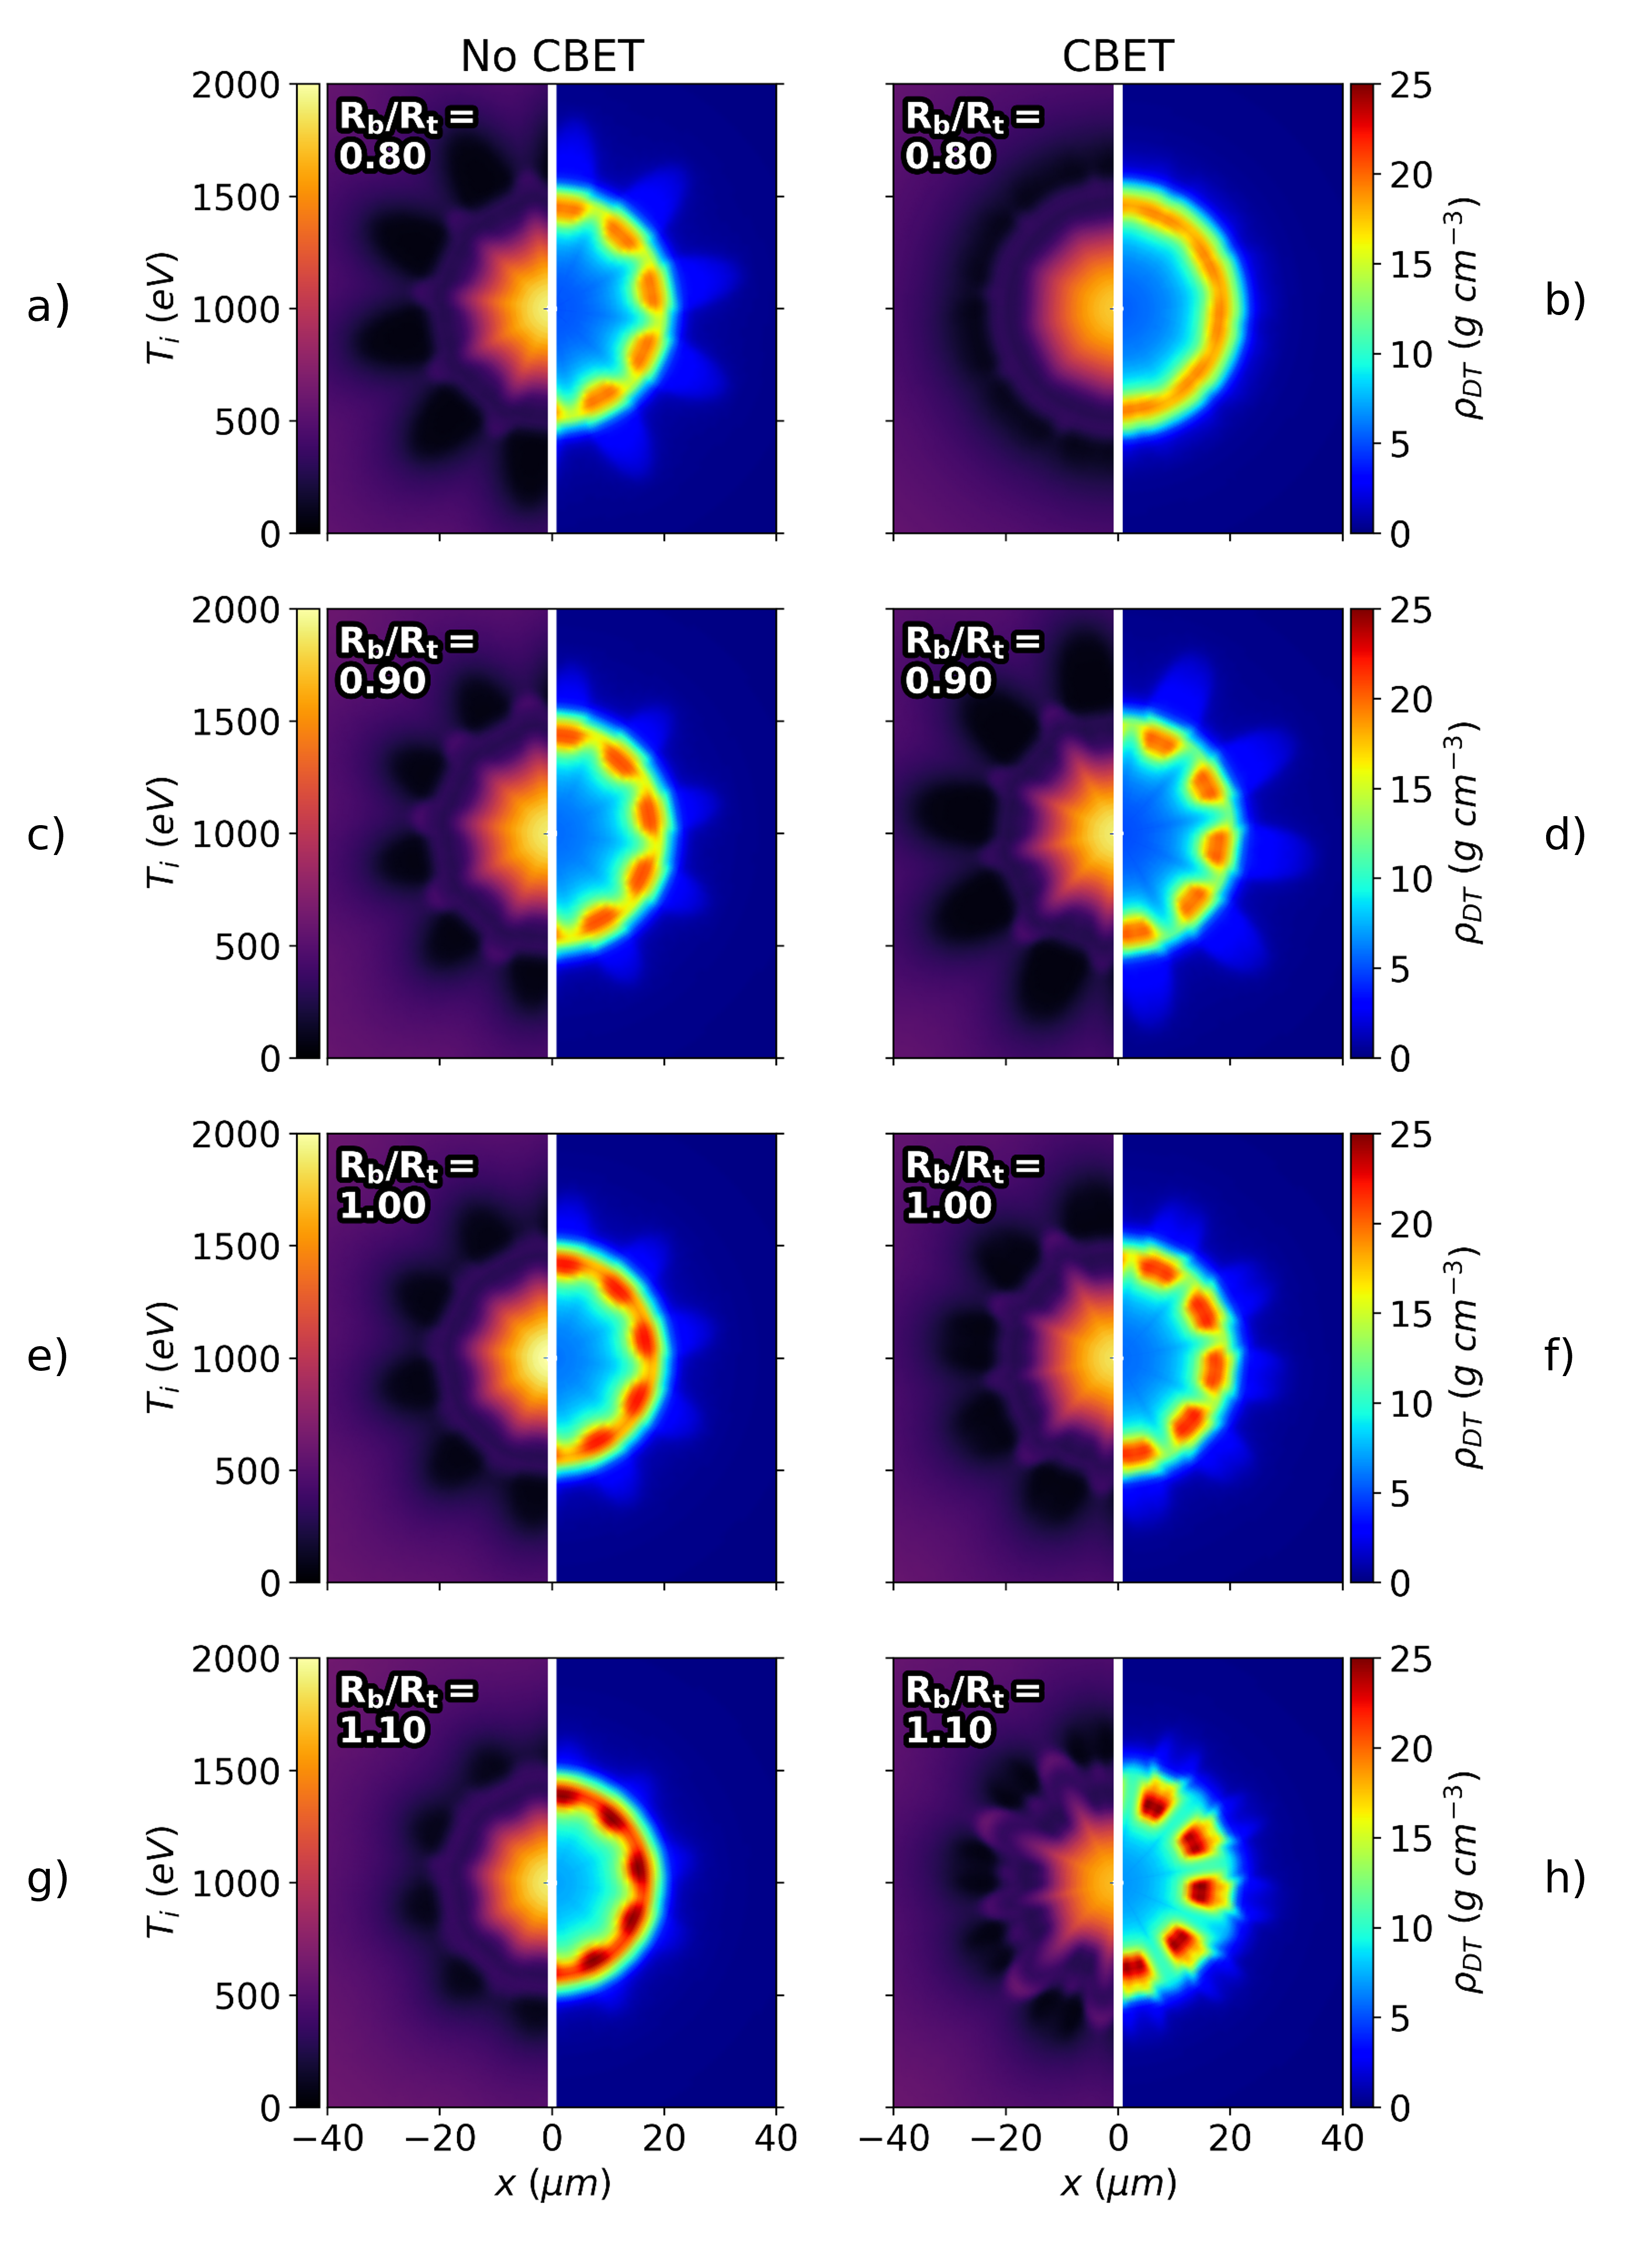
\includegraphics[width=0.9\linewidth]{Results1/Images/Stagnation_plots.png}
    \centering
    \caption{Densities of the DT fuel and ion temperatures for various $R_b/R_t$ simulations both with and without \ac{CBET}.
    Each row correspond to a different $R_b/R_t$ value; the left column contains simulations without \ac{CBET}; and the right column contains simulations with \ac{CBET}.
    It is visible from the density plots that increasing $R_b/R_t$ improves stagnation symmetry for the no \ac{CBET} simulations, but degrades it for the \ac{CBET} simulations.}%
    \label{fig:Res1_stagnation_plots}
\end{figure}



%################################################################################
%################################################################################
\subsection{Stagnation State Asymmetry Trend with Beam Radius}%
\label{sec:Res1_stagnation_asymm_trend}

\begin{figure}[t!]
    \includegraphics[width=1.0\linewidth]{Results1/Images/RbRt_sig_rhomax.png}
    \centering
    \caption{Trends of a) stagnation asymmetry and b) maximum (azimuthally averaged) fuel density for \ac{CBET} and no \ac{CBET} simulations.
    The no \ac{CBET} improvement in symmetry with $R_b/R_t$ is observed which also corresponds to improved compression.
    The symmetry trend including \ac{CBET} is more complex, but broadly the stagnation state symmetry is worse with increasing $R_b/R_t$.}%
    \label{fig:Res1_asymm_trend}
\end{figure}


%################################################################################
%################################################################################
\subsection{Time Resolved Asymmetry Growth}%
\label{sec:Res1_time_res_growth}

\begin{figure}[t!]
    \includegraphics[width=0.75\linewidth]{Results1/Images/RbRts_mode10_growth.png}
    \centering
    \caption{Time resolved $\ell=10$ Fourier power spectrum amplitude for a) $\rho_{\text{DT}}R$ and b) $P_{\text{dep}}R$ for \ac{CBET} simulations with 3 $R_b/R_t$ values.
    The developing but unrealised modal flip for $R_b/R_t=0.8$ from $t \sim 0.5\rightarrow 1.2\ \text{ns}$ reduces the $P_{\text{dep}}R_{\ell=10}$ leading to slow $\rho_{\text{DT}}R_{\ell=10}$ growth and ultimately a relatively symmetric stagnation state.
    %Note that this developing but unrealised modal flip is clearly visible from reduced $P_{\text{dep}}R$ asymmetry values in Fig.~\ref{fig:Res1_PR_CBET_modes}.a.
    Despite large values of $\rho_{\text{DT}}R_{\ell=10}$ initially, the developing modal flip of the $R_b/R_t=1.0$ simulation from $t \sim 1.8\rightarrow 2.1\ \text{ns}$ slows the density asymmetry growth.}%
    \label{fig:Res1_mode10_growths}
\end{figure}


%###############################################################################################################################
%###############################################################################################################################
%###############################################################################################################################
\section{Conclusions}%
\label{sec:Res1_Conclusions}


%################################################################################
%################################################################################
\subsection{Summary of work}%
\label{sec:Res1_Summary}


%################################################################################
%################################################################################
\subsection{Future Work}%
\label{sec:Res1_future}